\section{Actividad No 04 – Restricci\'on y Ordenamiento} 
		
\begin{enumerate}[1.]
	\item Debido a problemas con el presupuesto, el departamento de Recursos Humanos requiere un reporte que muestre los apellidos (last\_name) y salarios (salary) de todos los empleados que ganen más de \$ 12,000.
	\\ \\ select last\_name,salary from employees where salary > 12000;

	\begin{center}
	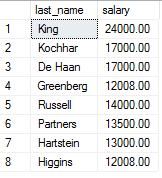
\includegraphics[width=5cm]{./Imagenes/actividad_04_01} 
	\end{center}

	\item Asimismo se requiere realizar una consulta que muestre los apellidos (last\_name) y el n\'umero de departamento (department\_id) para los empleados que tengan numero (employee\_id) 176.

	\begin{center}
	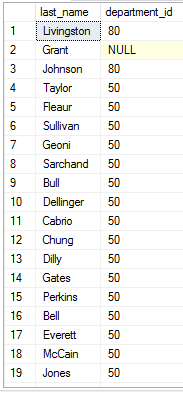
\includegraphics[width=5cm]{./Imagenes/actividad_04_02} 
	\end{center}

	\item El departamento de Recursos Humanos necesita determinar los mayores y menores sueldos, modificar la consulta del  ítem 4.1. para mostrar el apellido y salario de cada empleado cuyo sueldo no est\'e en el rango de \$ 5,000 a \$ 12,000.

	\begin{center}
	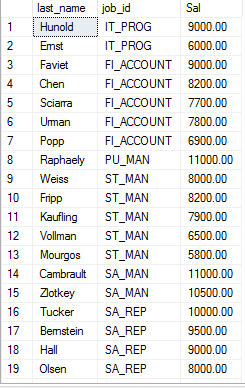
\includegraphics[width=5cm]{./Imagenes/actividad_04_03} 
	\end{center}

	\item Crear un reporte que muestre los apellidos (last\_name), puesto (job\_id) y fecha de contrataci\'on (hire\_date), de los empleados que apellidan ‘Matos’ y ‘Taylor’, asimismo presentar el reporte ordenado ascendentemente por fecha de contrataci\'on.

	\begin{center}
	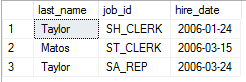
\includegraphics[width=5cm]{./Imagenes/actividad_04_04} 
	\end{center}

	\item Mostrar los apellidos (last\_name) y n\'umero de departamento (departamento\_id) de todos los empleados que pertenezcan a los departamentos 20 o 50 en orden alfab\'etico ascendente por el apellido.
	
	\begin{center}
	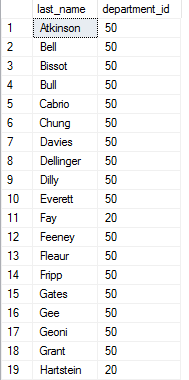
\includegraphics[width=5cm]{./Imagenes/actividad_04_05} 
	\end{center}
	
	\item Modificar el reporte del ítem 4.1. para mostrar los apellidos y salarios de los empleados que tengan un salario entre los \$ 5,000 a \$ 12,000 y pertenezcan a los números de departamento 20 o 50. Asimismo etiquetar las cabeceras de los resultados con los alias Empleado y Salario Mensual respectivamente.

	\begin{center}
	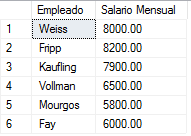
\includegraphics[width=5cm]{./Imagenes/actividad_04_06} 
	\end{center}

	\item El departamento de Recursos Humanos necesita un listado de apellidos (last\_name) y fecha de contrataci\'on (hire\_date) de todos los empleados que fueron contratados el año 1994.

	\begin{center}
	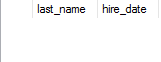
\includegraphics[width=5cm]{./Imagenes/actividad_04_07} 
	\end{center}

	\item Crear un reporte que muestre los apellidos (last\_name) y puesto (job\_id) de todos los empleados que
no tengan un administrador (manager).

	\begin{center}
	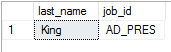
\includegraphics[width=5cm]{./Imagenes/actividad_04_08} 
	\end{center}

	\item Crear un reporte para mostrar los apellidos (last\_name), salario (salary) y \% de comisión (commission\_pct). Ordenar los datos por salario y comisión de manera descendente, utilizar la opción numérica de la cláusula ORDER BY.

	\begin{center}
	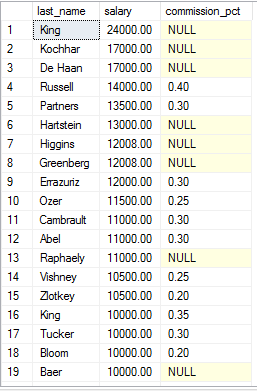
\includegraphics[width=5cm]{./Imagenes/actividad_04_09} 
	\end{center}


	\item El personal del departamento de Recursos Humanos desea tener mayor flexibilidad con los reportes hechos. Por ejemplo se requiere un reporte de los apellidos (last\_name) y salarios (salary) de todos los empleados que tengan un salario mayor a un monto que el personal de Recursos Humanos ingresará. Probar con el valor \$ 12,000

	\begin{center}
	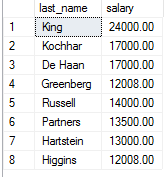
\includegraphics[width=5cm]{./Imagenes/actividad_04_10} 
	\end{center}

	\item El departamento de Recursos Humanos requiere extraer reporte basados en el Administrador (manager\_id). Se requiere crear una consulta que pregunte al usuario por el Administrador (manager\_id) y genere un reporte con los números de empleado (employee\_id), apellidos (last\_name), salarios (salary) y numero de departamento de los empleados que este Administrador tiene a su cargo. Adicionalmente también se desea tener la habilidad de ordenar este reporte en base a una determinada columna. Probar con los siguientes valores:
	\\Administrador (manager\_id) = 103, ordenado por Apellido (last\_name)
	\\Administrador (manager\_id) = 201, ordenado por Salario (salary)
	\\Administrador (manager\_id) = 124, ordenado por No de Empleado (employee\_id)

	\begin{center}
	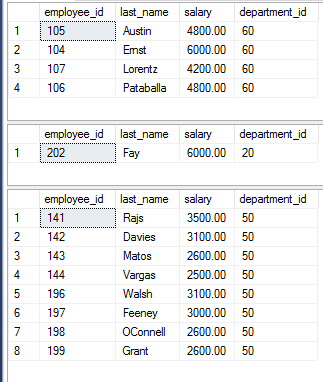
\includegraphics[width=5cm]{./Imagenes/actividad_04_11} 
	\end{center}

	\item Generar un listado de apellidos (last\_name) de todos los empleados que tengan la letra ‘a’ en la tercera letra de su apellido.

	\begin{center}
	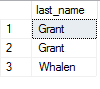
\includegraphics[width=5cm]{./Imagenes/actividad_04_12} 
	\end{center}

	\item Mostrar los apellidos (last\_name) de todos los empleados que tengan tanto la letra ‘a’ como la letra ‘e’
en su apellido.

	\begin{center}
	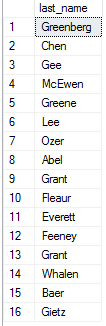
\includegraphics[width=5cm]{./Imagenes/actividad_04_13} 
	\end{center}

	\item Mostrar los apellidos (last\_name), puestos (job\_id) y salario (salary) de todos los empleados que sean Representantes de Ventas (SA\_REP) o Responsables de Inventario (ST\_CLERK) y cuyos salarios no sean iguales a \$ 2,500, \$ 3,500 o \$ 7,000.

	\begin{center}
	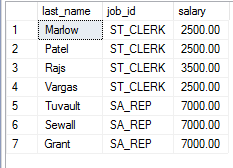
\includegraphics[width=5cm]{./Imagenes/actividad_04_14} 
	\end{center}

	\item Modificar el reporte del ítem 4.6 y mostrar adicionalmente los datos de comisión (commission\_pct) de
todos los empleados que solamente el 20\% de comisi\'on.

	\begin{center}
	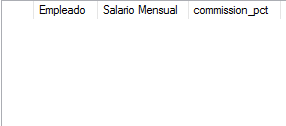
\includegraphics[width=5cm]{./Imagenes/actividad_04_15} 
	\end{center}

\end{enumerate}

